\chapter{Discussion and Future Work} 

%TODO fix informality

\section{Improved data gathering}
As we have shown above, increasing the amount of data is useful for training a more generalizable model.
Generating large biological datasets is difficult, but there is a movement towards greater automation of lab tasks.
In particular, we showed that a lab robot such as the Labcyte Echo can be used to generate larger scale datasets.
We encourage future work to take this even further and generate datasets with hundreds or even thousands of starting conditions.

\begin{figure}[t!]
\begin{center}
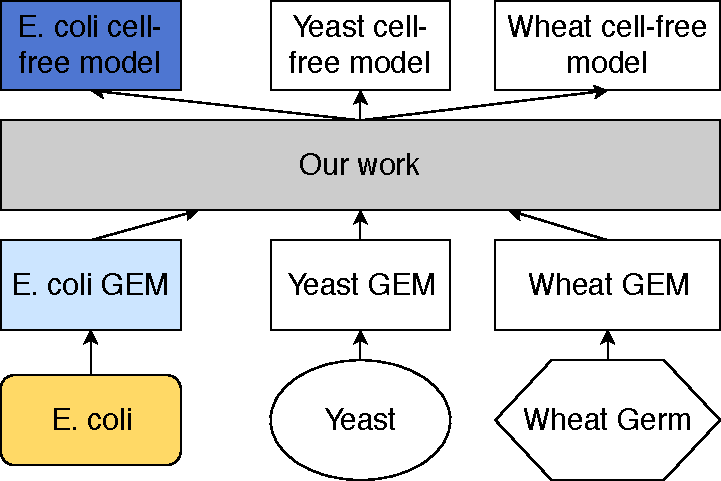
\includegraphics{figs/Vision.pdf}
\caption{Potential future usage for our system: converting different organism's \glspl{gem} into appropriate cell-free models.}
\end{center}
\label{fig:vision}
\end{figure}

\section{Different cell types}
We have only explored the usage of this technique on a \ecoli cell-free model.
However, there is a lot of work currently ongoing to use non-\ecoli cell-free models.
%TODO what needs to change to transfer to other organisms
This system was written with generalizability in mind and should transfer to other organisms as well.
In particular, this was the intent with creating a reduction system instead of hand-building a model from scratch.
There are dozens of \gls{fba} models of other organisms that this could be applied to.
Figure \ref{fig:vision} demonstrates our vision as a general purpose system for creating cell-free models.

In particular, the primary author of this work is a part of an Open Plant grant which involves the exploration of using wheat-germ cell-free systems.
The data is currently being generated through a collaboration with the Earlham Institute.
After the data generation is done, we want to apply this to that data to see its effectiveness.
%TODO explain
Additionally, this system will get a web interface to encourage other biologists to use it for their own data.

%TODO: talk about https://www.cell.com/cell-systems/pdf/S2405-4712(17)30010-8.pdf

\section{RL system for reduction}
One thing that we noticed while thinking about the best way to reduce the model is that we could frame the problem in terms of a reinforcement learning problem.
We originally tried to determine which reactions to remove by hand.
However, the way we went about this was to remove a reaction and re-run the model to see the output.
Then, we compared how well we match the experimental data.
So, we built a reinforcement learning framework to do this.
Rewards are based on how well our collection of models reflects the experimental data.

Simply doing a naive search with this RL framework would take far too long.
Starting with 2600 reactions, performing a random search over this space could take up to TODO.
Thus, we could use the \gls{vae} that we wrote in conjunction with this framework to perform a better directed search.
This could allow us to reduce the model even further and get even more specificity in the reduction.

\section{Improved starting model}
One potential issue that is limiting the usefulness of our pipeline is how well described the initial models are.
They're only as good as they are allowed to be by the reactions that exist.
\gls{fba} models undergo improvements periodically and we're using the most prominent model iJO1366.
However, as this model is updated, our model can adapt and use more up-to-date reactions.

\begin{figure}[t!]
\begin{center}
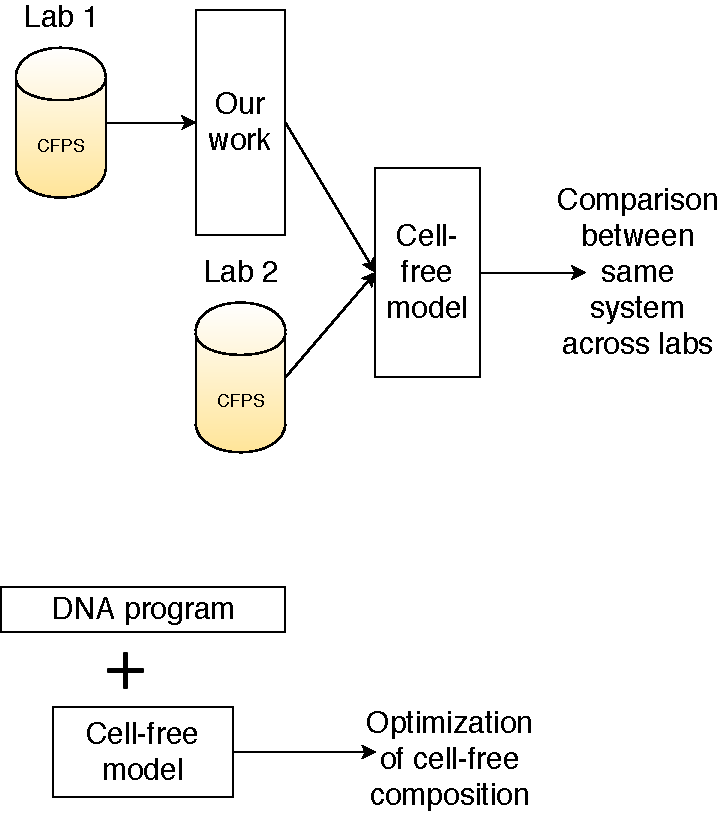
\includegraphics{figs/Applications.pdf}
\caption{Two future applications of our system.
Above, multiple experiments can be projected in the same subspace to better compare experimental results.
Below, the system can help optimize the energetic composition of a cell-free system}
\end{center}
\label{fig:apps}
\end{figure}

\section{Batch variation}
Batch variation is an important problem facing the cell-free community.
Some studies have shown up to 20\% variation between batches for the same protocols and \gls{dna} constructs.
This is an incredibly important issue because the typical workflow for a researcher may involve the characterization of a circuit through a series of different conditions or slightly different \gls{dna} programs.
However, most people need to compare the performance of these variations.
In order to deal with variation, researchers will perform all of their experiments with a single batch.
When that batch runs out, though, they will be required to re-characterize and redo all of the experiments they have already done.

Figure \ref{fig:apps} shows how our system provides a potential solution to this issue of batch variation.
A researcher runs a calibration set of experiments and then use those experiments to generate a \gls{vae} model based on that data.
Then, any future experiments that are performed (either in the same batch or a different one) could be projected into the same latent space in order to allow comparison between the experiments.
This would allow the translation of all of the data generated into the same subspace and allow better comparisons across batches.

%TODO: fix conclusion
In conclusion, we have shown that deep learning techniques can be successfully applied to biology.
In particular, computational biologists should start using \glspl{ae} (especially \glspl{vae}) for dimensionality reduction instead of automatically defaulting to using \gls{pca}.
The loss function that we developed for our \gls{vae} is general enough to be used with any form of biological data.
We hope this work encourages other computational biologists to continue work integrating deep learning with biology in general and metabolic models specifically.